\chapter{Implementação}

A solução encontra-se dividida em vários projetos de bibliotecas, aplicações de consola e uma aplicação WinForm. 

\section{Central Manager} \label{seccentralmanager}

Para ser implementado o servidor central, foi necessário definir a interface ICentralManager, apresentada na figura \ref{icentralmanager}.\\ 

\begin{figure}[h]
	\makebox[\textwidth][c]{
		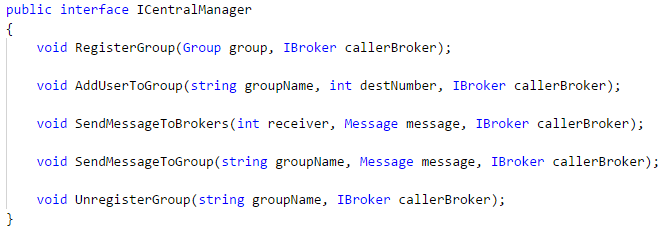
\includegraphics[width=1.0\textwidth]{./figures/icentralmanager}
	}
	\caption{Interface ICentralManager}
	\label{icentralmanager}
\end{figure}

O \textit{central manager} conhece todos os servidores regionais existentes, pois é injetado no construtor uma lista com todos os \textit{proxies} dos servidores regionais desse sistema. Desta forma, o \textit{central manager} é \textit{stateless} visto que não armazena mais nenhuma informação.\\

Para a implementação do \textit{central manager}, foi usado o padrão \textit{singleton}. O padrão \textit{singleton} adequa-se melhor às necessidades, pois assume-se que o servidor central estará sempre a receber e a enviar pedidos. Desta forma o padrão \textit{single call} teria muito maior \textit{overhead} em relação ao \textit{singleton} pois teria de estar sempre a criar novas instâncias para responder a cada pedido, sendo que não se sabe o número de pedidos de antemão.\\

De modo a que não é possível determinar o uso deste sistema distribuído, não existe forma de saber se é usado com bastante regularidade e com espaçamento no intervalo de tempo entre as mensagens; No pior dos casos tem o objeto em memória com tempo infinito e os pedidos nunca passam pelo \textit{manager}, e no melhor dos casos os pedidos são atendidos sempre pela mesma instância, sem esta estar a ocupar recursos em memória desnecessariamente.\\

O \textit{lease time} escolhido para a instância do \textit{central manager} foi o tempo por omissão do CLR do .NET que é de 5 minutos e o tempo de renovação por cada chamada é também de 5 minutos. Foi tomada essa decisão porque não é possível prever o intervalo de tempo entre cada mensagem consecutiva. O problema com esta decisão é se o intervalo entre cada mensagem for superior a 5 minutos. Isto irá causar o \textit{overhead} da criação do \textit{manager}. A vantagem desta solução é que se o intervalo entre as mensagens for superior ao dobro do tempo de renovação, não ocupa recursos desnecessariamente.

\section{Broker} \label{broker}

Para implementar o servidor regional, definiu-se duas interfaces. A interface para interação com o utilizador é IBrokerService, apresentada na figura \label{ibrokerservice}. 

% METER FIGURA IBrokerService

A interface para a interação com o \textit{central manager} é IBrokerClient, apresentada na figura \label{ibrokerclient}.

% METER FIGURA IBrokerClient

O \textit{broker} mantém informação dos utilizadores registados nessa região e dos grupos existentes em todas as regiões. Desta forma, o \textit{broker} é \textit{stateful}.\\

Para a implementação do \textit{broker} foi usado o padrão \textit{singleton}. Foi usado este padrão, pois existe a necessidade de manter estado. Se fosse usado o padrão \textit{single call}, tal não era permitido porque seria criado uma instância por cada pedido, impossibilitando a agregação de informação.\\

O \textit{lease time} escolhido foi zero, o que significa que este terá um tempo de vida infinito. Isto porque devido à necessidade de manter estado, se fosse chamado o desconstrutor da instância, perdia-se toda a informação sobre os utilizadores e grupos.
